\chapter{From the horizon to the nucleus}\label{ch:bridge}

\section{Astro-Genetics}

\emph{Astro-Genetics} is our name for one idea: read the methylome the way
cosmology reads the sky. A telescope records the brightness of the cosmic microwave background
(CMB) at millions of directions; after calibration and component separation, what remains is a map
whose small variations carry the physics of the early universe. A methylation array records the
methylated fraction $\beta$ at hundreds of thousands of CpG positions; after calibration and
deconvolution, what remains is a set of cells, each with a methylation state that carries the
physics of that cell. The measurement problems are the same kind of problem: a noisy instrument, a
signal mixed from many sources, and a need to separate what is known from what is new. So the
tools are the same tools.
Cosmology was forced by its data to build a toolkit for reading one system against a calibrated reference and saying how far it sits from
where it should be. Astro-Genetics hands that toolkit to the cell. The work is cartography: we map what is there. We do not invent the
territory; we find it and chart it. The CpG sites are already there, and so is the healthy reading of each cell type, waiting to be
measured. Stargazers see what is there; trailblazers go where no one has been. Astro-Genetics does both at once: it reads the methylome
with instruments the sky has already proved, and it reads each cell against a floor set by physics. \analogy

That is the methodological half of the bridge, and it stands without any new physics. Chapter~\ref{ch:skytools} is
devoted to it. The physical half is a stronger claim, and it is the subject of this Part: that the
cost which governs an encoding surface in cosmology governs the methylome too.
\paragraph{The energy that holds it.} A cell keeps its identity written in its DNA: not in the genes themselves, but in methyl groups placed
on cytosines at specific sites along the strand. The pattern is copied at every division by an enzyme of finite fidelity, and thermal noise
at 310~K works to scramble it. Holding the pattern costs energy, and the price per bit is the same $\kB T\ln2$ a horizon charges. On single
molecules of healthy cells the energy that holds each maintained site against that noise is $3.41\,\kB T$ (Chapter~\ref{ch:landauer}).
\measured{} The methylation pattern is the cell's running ledger of what kind of cell it is, and the gauge of this Part reads how well
the ledger is kept.

If every cell maintains its identity by paying a continuous cost against the noise that would randomize it, then life itself comes into view
as the continuous purchase of organized pattern, sustained by metabolic work against the second law. Schr\"odinger asked the same question in
1944~\cite{SchrodingerWhatIsLife}. We raise it here and leave it open. \interp

\section{One cost, many surfaces}

A cell is a microchip. Each cell type runs its own program, written as a pattern of methylated and unmethylated sites, and it pays energy
to keep that program from being overwritten by noise. A neutrophil runs the neutrophil program, a neuron the neuron program, and each is read
against itself. The methylation pattern is the cell's notebook: the place where it writes down what kind of cell it is, so that the next copy
can read it back after division. A notebook that is kept well can be read; one that is written over carelessly becomes noise. \analogy


Landauer's principle states that erasing one bit of information in contact with a reservoir at
temperature $T$ dissipates at least~\cite{Landauer1961,Bennett1982}
\begin{equation}
  E_{\mathrm{bit}}=\kB T\ln 2 .
  \label{eq:landauer}
\end{equation}
It has been measured directly on a colloidal particle in a double well~\cite{Berut2012} and on
nanomagnets~\cite{Hong2016}. Nothing in Eq.~\eqref{eq:landauer} refers to what the bit is made of.
The same expression, evaluated at the Hawking temperature, is the cost per bit on a black-hole
horizon; evaluated at 20~mK it is the cost per bit in a superconducting qubit; evaluated at
310.15~K it is the cost per bit in a cell nucleus (Figure~\ref{fig:landauerT}).

\begin{figure}[htbp]\centering
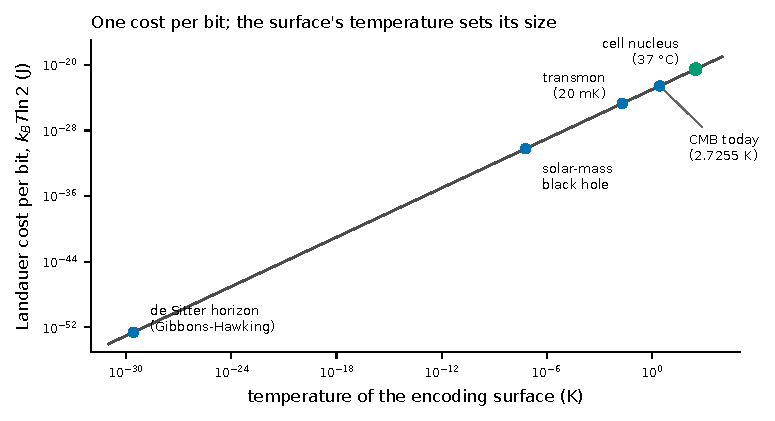
\includegraphics[width=0.9\textwidth]{figures/part4/fig_landauer_temperatures.pdf}
\caption{The Landauer cost per bit, $\kB T\ln2$, at the temperatures of the encoding surfaces
discussed in this book. The de~Sitter horizon uses the Gibbons--Hawking
temperature $\hbar H_0/2\pi\kB$ with $H_0=67.4$~km\,s$^{-1}$\,Mpc$^{-1}$ (Planck 2018, base $\Lambda$CDM~\cite{Planck2018VI}); the black hole is one
solar mass. \calc}
\label{fig:landauerT}
\end{figure}

IAM's Law (Chapter~\ref{ch:iams_law}) states the one identification the framework adds to that textbook statement:
every irreversible transition from quantum superposition to classical record pays $\kB T\ln2$ per bit to the
\emph{nearest encoding surface} of the system doing the writing, at that surface's own temperature. \conjecture For a horizon the
surface is the horizon; for a qubit it is the junction and its substrate; for a transistor it is
the gate; for a cell it is the chromatin on which the methylation pattern is written and
maintained. Parts~\ref{part:2} and~\ref{part:3} test this identification in cosmology, particle physics and
quantum hardware, and label each result by how well it holds. This part tests it on the cell.

\section{What the bridge claims, and what it does not}

\paragraph{Why your cells follow the same law as the stars.} Anything that lasts holds a balance between the energy of motion and the energy
that holds it together. For a star, a galaxy or an atom bound by a $1/r$ force, the balance is exact: the kinetic energy is half the binding
energy (Chapter~\ref{ch:virial_law}). \derived{} A cell is held together by chemistry, not by gravity, so the half does not carry over as a
number; what carries over is the accounting. The cell spends energy to hold its pattern against thermal noise, and the price per bit is the
same $\kB T\ln2$ (Chapter~\ref{ch:landauer}). \derived{} The claim that the cell's maintenance balance is the same balance as a star's is
interpretation. \interp


It is worth being exact at the outset, because the bridge is easy to overstate.

\begin{keybox}[title=What the bridge claims]
\begin{enumerate}
\item The Landauer cost per bit applies to the maintenance of a methylation pattern, as it applies
      to any irreversible write. \derived
\item A cell's methylation pattern is held by a copying process of finite fidelity, and that fidelity can be read: on
      arrays as the entropy of the pattern on the sites that make the cell what it is, against the same cell type's healthy
      reading (\calibrated, Chapter~\ref{ch:meta}); on single molecules as the copy error, against a floor whose form follows
      from a Boltzmann factor (\derived) and whose height is measured (\measured, Chapter~\ref{ch:iama}).
\item The analysis tools that separate a known foreground from a signal on the sky separate known
      cells from a new signal in a blood draw. \analogy{} of structure; each tool is then tested on
      its own (Chapter~\ref{ch:skytools}).
\end{enumerate}
\end{keybox}

\begin{keybox}[title=What the bridge does not claim]
\begin{enumerate}
\item It does not claim that a cell and a black hole have the same numbers. A solar-mass horizon
      holds $1.5\times10^{77}$ bits at $6.2\times10^{-8}$~K; a cell's methylome holds about
      $2.8\times10^7$ at 310~K (Figure~\ref{fig:scaleladder}). The bit counts differ by 70 orders
      of magnitude and the temperatures by ten. The equation is shared; the parameters are not.
\item It does not yet derive the height of the cell's floor $\Hmin$ from first principles. Its form is a Boltzmann
      factor; its height comes from the holding energy measured on healthy molecules. Deriving that energy from the
      chemistry of maintenance is the framework's central open problem at cellular scale (Chapter~\ref{ch:open}).
\item It does not use any population of people to define what a cell should read.
\end{enumerate}
\end{keybox}

\begin{figure}[htbp]\centering
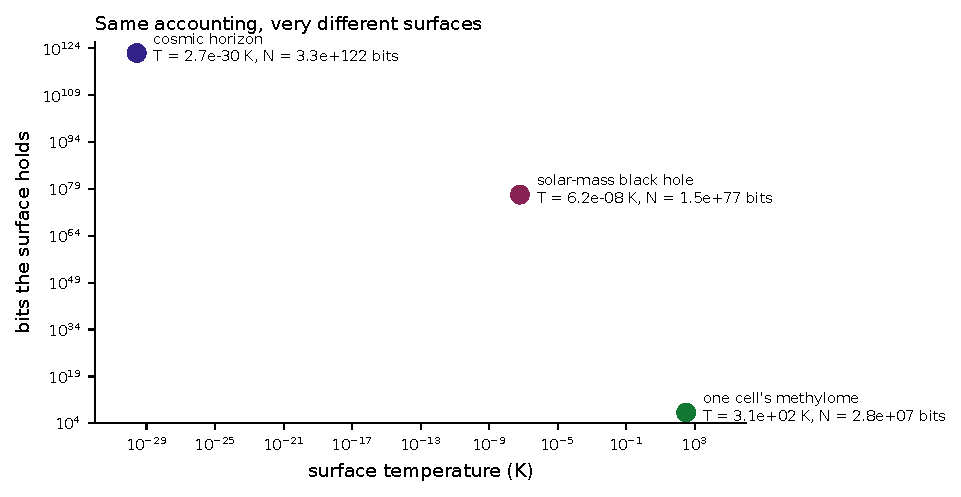
\includegraphics[width=0.78\textwidth]{figures/part4/fig_scale_ladder.pdf}
\caption{Three encoding surfaces by temperature and capacity. Cosmic horizon: Gibbons--Hawking
temperature and area$/4\lP^2$ at the Hubble radius. Solar-mass black hole: Hawking temperature
and Bekenstein--Hawking entropy. Cell: body temperature and one bit per CpG on one strand of a
hg38 genome ($\sim$28 million). \calc}
\label{fig:scaleladder}
\end{figure}

\section{Thirty-seven orders of magnitude}

The phrase ``37 orders of magnitude'' recurs throughout this book. It refers to the span of
length from an atom ($\sim10^{-10}$~m) to the cosmic horizon ($c/H_0\approx1.4\times10^{26}$~m),
which is 36.1 orders, or from the Bohr radius to the particle horizon, which is closer to 37.
The claim it carries is that the same accounting applies across that span. It is a claim about
range, not about a single measurement, and each rung of the range is tested separately: the
horizon rungs in Part~\ref{part:2}, the devices in Part~\ref{part:3}, the cellular rung here.

Table~\ref{tab:p4_surfaces} puts the shared equation and the different parameters side by side for four surfaces. The cost per bit
depends only on the temperature; the capacity, where it is defined, sets the cost of holding the whole surface. \calc

\begin{table}[htbp]\centering\small
\caption{Four encoding surfaces on one equation, $E_{\rm bit}=\kB T\ln2$. Horizons: Hawking temperature and Bekenstein--Hawking capacity
$S/(\kB\ln2)$; cell: one bit per CpG copy of one haploid genome (Chapter~\ref{ch:surface}). \calc{} (CODATA constants; \texttt{figscripts/fig\_p4.py --tables}).}\label{tab:p4_surfaces}
\begin{tabular}{@{}lrrrr@{}}\toprule
surface & $T$ (K) & $\kB T\ln2$ (J) & capacity (bits) & full surface (J) \\\midrule
horizon, one solar mass & $6.2\times10^{-8}$ & $5.9\times10^{-31}$ & $1.5\times10^{77}$ & $8.9\times10^{46}$ \\
horizon, $10^6$ solar masses & $6.2\times10^{-14}$ & $5.9\times10^{-37}$ & $1.5\times10^{89}$ & $8.9\times10^{52}$ \\
superconducting qubit, 20 mK & $2.0\times10^{-2}$ & $1.9\times10^{-25}$ & one per qubit & --- \\
cell nucleus, 310.15 K & $3.1\times10^{2}$ & $3.0\times10^{-21}$ & $2.8\times10^{7}$ & $8.3\times10^{-14}$ \\
\bottomrule
\end{tabular}
\end{table}

\section{How the framework was built, and why that matters for a reader}

The framework was not built on the cell first. It was built on the horizon, where the entropy
functional of a causal surface is tractable (Jacobson's derivation of the Einstein equation from
the Clausius relation~\cite{Jacobson1995}, extended by an informational term). It was then carried
to substrates where the same structure should appear in different physical clothing:
semiconductor logic, superconducting and trapped-ion qubits, and finally methylation. The method has
four steps:
\begin{enumerate}
\item identify a thermodynamic--informational invariant where a first-principles derivation is
      tractable;
\item test it against observations never used to build it;
\item identify substrates where the same structure should appear, and write down what the
      invariant becomes in each;
\item test each substrate against data that carry no information about the answer.
\end{enumerate}
The fourth step is the one this Part is most concerned with, because it is where methylation work
is most easily contaminated. A classifier trained on one set of specimens to separate groups learns whatever
distinguishes that set, and may or may not transfer. A physical reading of a cell against its
floor does not learn from other specimens, and so it cannot be selectively right: if the floor is wrong,
the reading is wrong everywhere. That is what makes it testable, and it is why the instrument of
this Part refuses every number that a panel of other people would supply.

The framework grew out of fifteen years of operating power generation and transmission
systems, where energy accounting and the failure of systems that cannot pay their costs are daily
practice. That background shaped the framework's emphasis on budgets, margins and failure walls.
It is stated here because it explains the vocabulary, not as evidence.

\section{The plan of Part~\ref{part:4}}

Chapter~\ref{ch:landauer} puts numbers on the cost at body temperature and defines the Mahaffey
number. Chapter~\ref{ch:surface} treats the methylome as an encoding surface and introduces binary
entropy. Chapter~\ref{ch:ledgers} states precisely what the virial theorem's one half does and does not say, and why
nothing in the gauge depends on it. Chapter~\ref{ch:floorbreach} sets a full horizon beside a cell whose pattern has
reached its own capacity, and separates the structural statement from the numerical one.
Chapters~\ref{ch:gauge} to~\ref{ch:temperature} build the gauge and its two readings, Chapters~\ref{ch:translation}
to~\ref{ch:chain} build the instrument that makes them, and the remaining chapters report the first readings and what is
established.
